\section{Versorgung und Einschaltung}

Es ist vorgesehen, das Gerät mit 24V Gleichspannung zu betreiben.
Dafür ist eine Buchse links an der vorderen Seite des Gehäuses herausgeführt.
Um den Raspberry Pi zu starten, braucht das Gerät nur an den passenden Stecker angesteckt werden.

\section{Buchsen für die Sensorschnittstellen}

Datenblatt: \url{https://xonstorage.blob.core.windows.net/pdf/cixikefa_jh1712p4p_xonjuly20_12_link.pdf}\\[0.5cm]
Es sind 4 Buchsen des Typs JH1710S-4P an der Vorderseite des Geräts herausgeführt, jeder davon kann einen Sensor auslesen.

\subsection{Pinbelegung}
Die Stecker verfügen über 4 Pins (nummeriert von 1 bis 4), davon sind aber nur 3  belegt (24V DC Versorgung, 4-20mA Datenleitung, GND).

\begin{itemize}
    \item Pin 1: Versorgung 24V DC (rotes Kabel im Gerät)
    \item Pin 2: GND (schwarzes Kabel im Gerät)
    \item Pin 3: Datenleitung 4-20mA (weißes Kabel im Gerät)
    \item Pin 4: offen
\end{itemize}



\subsection{Nenndaten}

\begin{itemize}
    \item Nennstrom: 5A
    \item Nennspannung: 200V
\end{itemize}

\section{USB-Port}
Um die ausgewerteten Daten des Geräts speichern zu können, befindet sich auf der linken Seite des Geräts eine USB-Buchse.

\newpage
\begin{figure}[h]
    \centering
    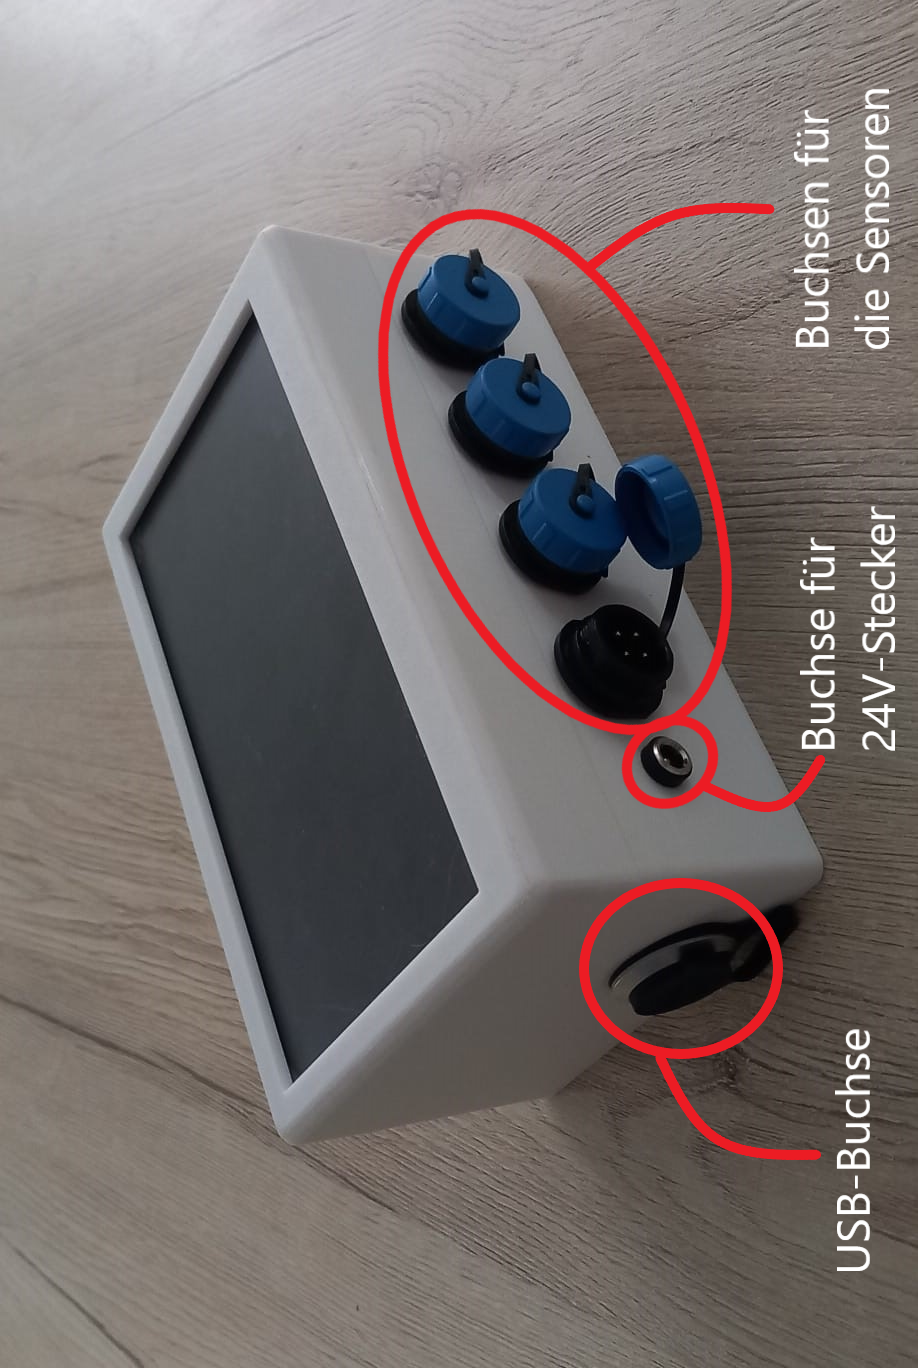
\includegraphics[width=0.9\linewidth]{Images/Gehause.bmp.png}
    \caption{Alle Buchsen des Gehäuses}
    \label{fig:Buchsen}
\end{figure}